\subsection{Non-Goals}
\begin{itemize}
\item Our goal is not to find the root cause of component failures; we're only interested in how the distributed system reacts to those failures (lightning strike example). Another way of putting this is that we aren't interested in troubleshooting anything outside of the controller software: if you have a bug in your switch, you should contact your hardware vendor; if you have a bug in your policy specification, take a closer look at what you specified; if you encounter a bug in your OS, get out your kernel debugger. (That said, our tool can tell you whether your switches behave the same as our software implementation: if our tool was unable to reproduce the error, that means that the problem was above or below the control software)
\item We don't aim to reproduce bugs involving non-determinism within a single controller (e.g. race-conditions between threads); we're interested in coarser granularity errors (e.g. incorrect failover logic), which there are plenty of! That said, if the developer is willing to instrument their system to provide finer granularity log messages (e.g. Gautam's Friday), our approach still applies.
\item We won't always find the globally minimum causal sequence, since that
would require $O(2^N)$ computation in the worst case. Our algorithm is however guaranteed to find a 1-minimal (locally minimum) causal sequence, meaning that if any event from the sequence is pruned, no persistent correctness violation occurs.
\item Primarily focused on correctness bugs, not performance bugs -- although this distinction has more to do with invariant checking than MCS finding.
\end{itemize}

\subsection{Algorithm}

Before presenting our approach, we describe an example bug in the Floodlight
open source control platform~\cite{floodlight_bug}. Floodlight is distributed across
multiple controllers for high availability, and provides support for
virtualization. Switches maintain one hot connection to a master controller and
several cold connections to replica controllers. The \emph{master} holds the
authority to issue state changing commands to the switches. The other
controllers are in \emph{slave} mode and do not perform any changes to the
switch configurations unless they detect that the master has crashed.

\begin{figure}[t]
    %\hspace{-10pt}
    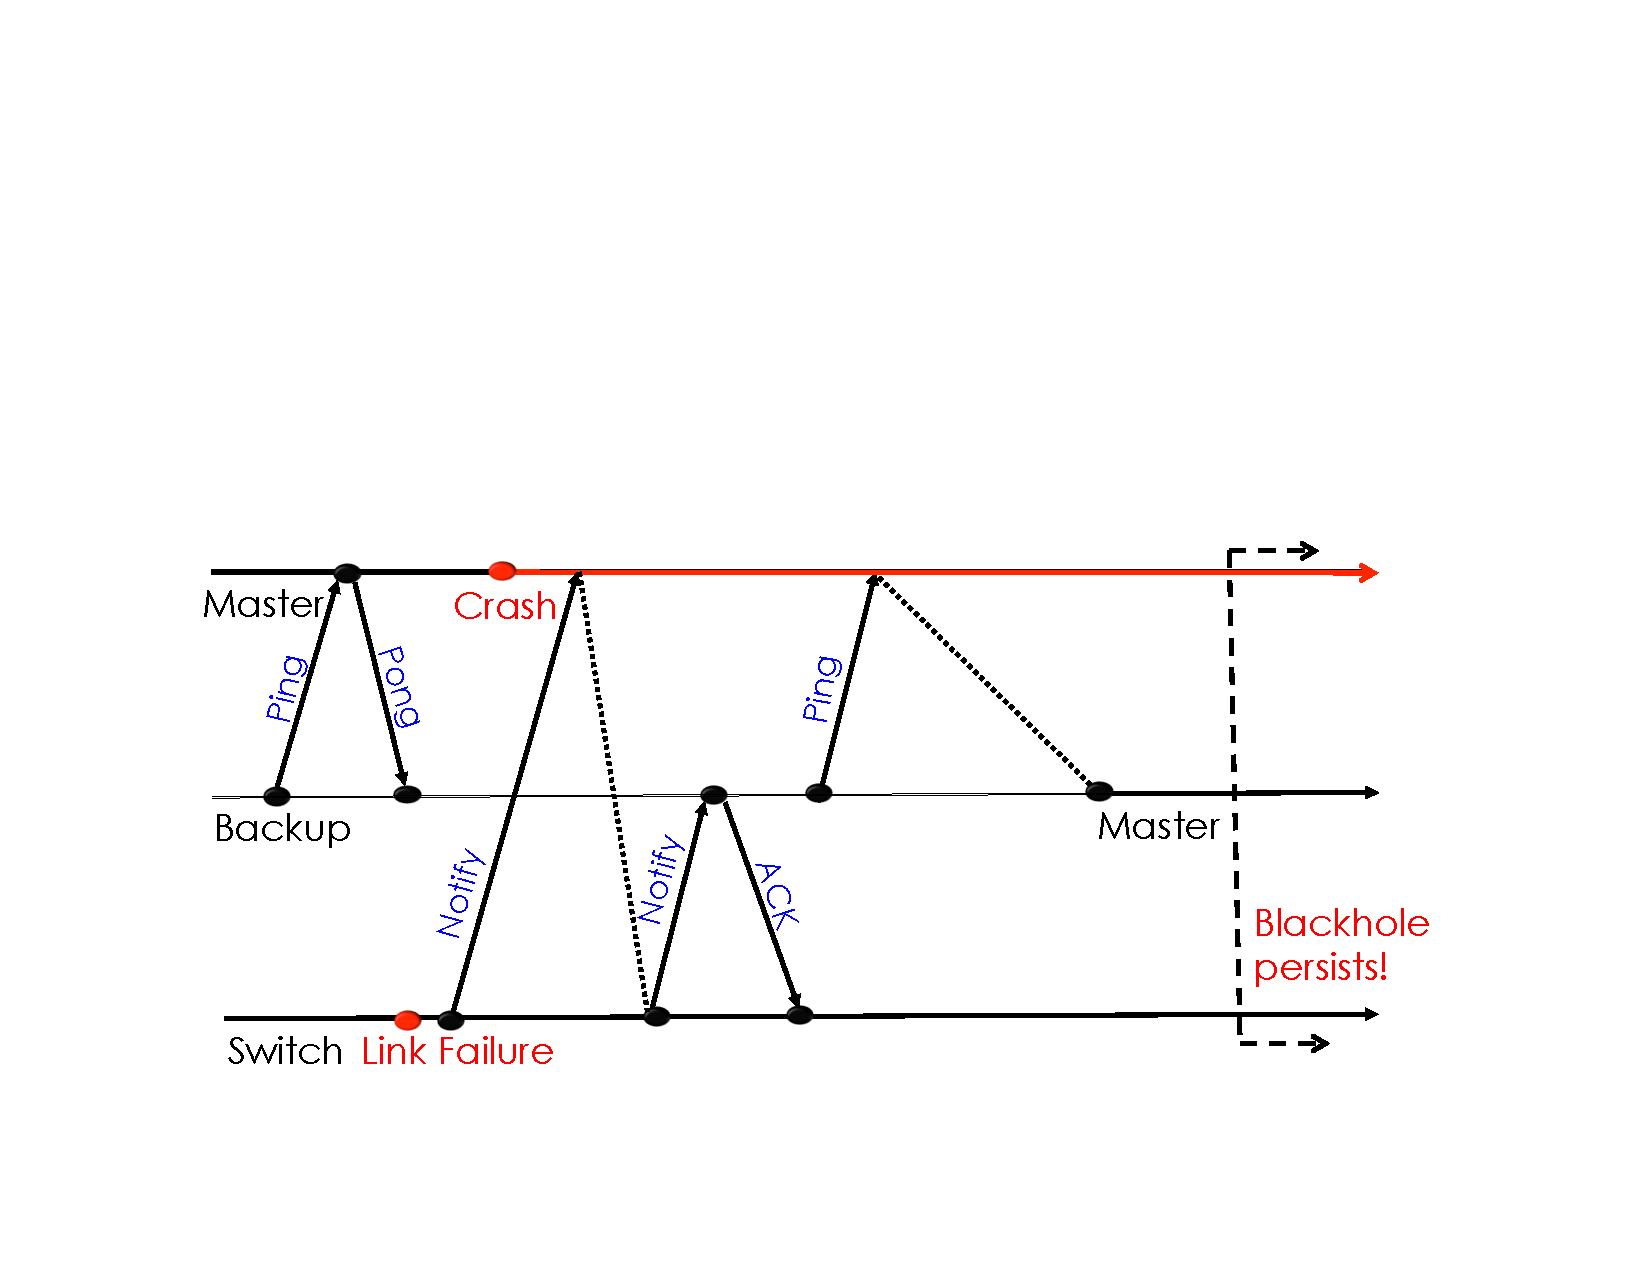
\includegraphics[width=3.25in]{../diagrams/case_study/example_bug.pdf}
    \caption[]{\label{fig:example} Floodlight failover bug. External inputs
               are depicted as red dots, internal events are depicted as black
               dots, and timeouts are depicted as dotted messages lines.}
\end{figure}

The failover logic in Floodlight is not implemented correctly, leading to the
following race condition\footnote{Note that this issue was
originally discovered by the developers of Floodlight~\cite{floodlight_bug}} depicted in
Figure~\ref{fig:example}:
a link fails (E1), and the switch attempts to notify the controllers (E2,E4) shortly after the master
controller has died (E3), but before a new master has been selected (E6). In this case, all live controllers are in
the slave role and thus will not take responsibility for updating the switch
flow table (E5). At some point, the heartbeats time out and one of the controllers
elevates itself to the master role (E6). The new master will proceed to manage
the newly connected switch, but without ever clearing the routing entries for
the failed link (resulting in a persistent blackhole).

There were only two external inputs (E1,E3) shown in our example.
Production datacenter logs contain
a significantly larger number of hardware failures, topology changes,
and other potential triggering events,
all of which may appear characteristic of normal operating
conditions at first glance; assuming 8.5 network error events per
minute~\cite{Greenberg:2009:VSF:1592568.1592576}, 500 VM migrations per
hour~\cite{Soundararajan:2010:CBS:1899928.1899941}, and a relevant execution
history of one hour, there would be over 1000 extraneous inputs to the system
reflected in the log.

Given a log of the system execution similar to the Floodlight case,
our goal is to prune events that are not
necessary for triggering errant behavior. We define errant behavior in terms
of {\em correctness violations}:
configurations of the network that are inconsistent
with the policy. In the example, the correctness violation is between a
reachability policy specified in the logical view (``A can talk to B'')
and the blackhole in the physical network (``A's packets to B enter the
blackhole and do not arrive at B'').

We have developed a technique to automatically perform this pruning.
Specifically, our technique identifies a minimal set of inputs
to the controllers that is sufficient for triggering a known correctness violation. We
refer to such inputs as a {\em minimal causal sequence} (MCS). Going back to our example,
suppose the log includes many more (extraneous) inputs. Whenever an
extraneous event is pruned, the blackhole will still persist. When
the controller crash is pruned, the blackhole will be resolved properly, and
when the link failure is pruned, no blackhole will occur. The MCS returned
is therefore the controller crash and the link failure in conjunction.

Delta debugging~\cite{Zeller:2002:SIF:506201.506206}, a technique from the
software engineering community, gets us part of the way
there: given a single input (\eg~an HTML page)
for a non-distributed program (\eg~Firefox), it performs a divide-and-conquer
search, repeatedly running the program on subsets of the input
until it finds a minimal subset (\eg~a {\tt<SELECT>} tag) that is sufficient
for triggering a known bug. \colin{Needs a figure.}

Our problem differs in two dimensions. First, the input to SDN controllers is spread
across time: it includes many messages, and depends on subtle causal
relationships. Second, the input is spread across space: it involving
many nodes which run asynchronously and may fail at any time.

The crux of our contribution lies in extending the delta debugging technique
to a distributed setting. In the rest of this section, we describe how we (i)
cope with alterations to the causal history of an execution and coordinate
replay across the distributed nodes in SDN networks, as well as (ii)
develop a generic invariant checking algorithm
for detecting errant behavior. In Section 4, we describe concrete ways in
which the technique can be put to use.

\subsection{Replay}
\begin{itemize}
\item It's not sufficient to replay the remaining inputs based only on the timings from the original log [we tried!]
\item So we incorporate events that are internal to the system under test (e.g. mastership changes), whose causal parents/children we don't explicitly know but can infer, as indicators of when we should inject external inputs (e.g. link failures), whose causal parents we don't know and will never know.
\item We interpose on the controllers' logging library and control message channels to get access to those internal events.
\item Note that the developer must provide enough logging statements so that relevant internal state changes are captured and visible to our tool. The logging statements must also contain enough context[d] to allow for unambiguous fingerprinting.
\item Naive solution: wait for internal events, but time out on those that don't show up. Problem: might wait too long. 
\item Soundest solution: peek()
  \begin{itemize}
    \item Infer which internal events are/aren't going to occur, so we know exactly how long to wait before injecting
    \item How do we know how far to peek() ahead?
    \item What to do about multiple matching fingerprints?
    \item overall $O(N^3)$ runtime--snapshots make it $O(N^2)$
  \end{itemize}
\item We apply domain knowledge to ensure validity of input sequences. For
example, it doesn't make sense to replay a link recovery event if we pruned
the link failure event that preceded it. Note that it's really hard to codify
the dependencies between some input events (e.g. dataplane drops). See gdoc
for a discussion.
\item In S4, we discuss some of the implementation details of handling internal events
\end{itemize}
\subsection{Correspondence Checking}
% Andi: keep concise
\begin{itemize}
\item We need a way to check at the end whether the violation has occurred. We call such an algorithm a decider. 
\item Here we present one decider: correspondence checking. 
\item Note that if you don't want to instrument controller, or your controller doesn't have an explicit view, you can also specify your own correctness conditions (e.g. reachability) 
\item Overview of HSA
\item We extract correctness specification directly from virtual view / physical view
\item Mathy math
\item Clarify that correctness violations are unambiguous -- if they were ambiguous, we might falsely prune a member of the MCS (bad!)
\item Shortcomings of CC
  \begin{itemize}
    \item doesn't help with performance (e.g. load balancing over internal links)
    \item assumes that policy specifications themselves are correct
  \end{itemize}
\end{itemize}


% ---------------------------------------------- %
%             OLD TEXT
\eat{

%Platform developers may discover correctness violations
%through customer complaints, integration tests, or by periodically running
%invariant checks on a deployed network.


\subsection{\SIMULATOR{}}
\label{sec:causal_analysis}

We have developed an algorithm, \simulator{}, for automatically inferring the inputs to the
controllers that are both necessary and sufficient for triggering the correctness violation. We
refer to these events as the {\em minimal causal sequence} (MCS). We show
the algorithm here, and elaborate in later sections:

\begin{Verbatim}[commandchars=\\\{\}]
Input: E = [e\textsubscript{1}, e\textsubscript{2}, e\textsubscript{3}, e\textsubscript{4}, ... e\textsubscript{n}]
Output: MCS

MCS = []
for i in 1 to n:
  if violation in replay(E - e\textsubscript{i}):
    E := E - e\textsubscript{i}
  else:
    MCS := MCS || e\textsubscript{i}
\end{Verbatim}

\noindent In words, the algorithm takes in a log of the system execution,
prunes each external input in isolation,
runs the system forward with the remaining input, checks whether the
correctness violation is still present, and thereby infers whether that input is
necessary for triggering the fault. Going back to our example, suppose the
log includes many more (extraneous) inputs. Whenever an
extraneous event is pruned, the blackhole will still persist. When
the controller crash is pruned, the blackhole will be resolved properly, and
when the link failure is pruned, no blackhole will occur. The MCS returned
is therefore the controller crash and the link failure in conjunction.

The crux of our contribution lies in specifying exactly how each
individual step of this algorithm works. In the rest of this section we will
describe our efforts to support \simulator{}, including (i)
detailing how execution logs are obtained
and what properties they need, (ii) developing a deterministic network simulator
to replay the execution of control software, and (iii) developing an invariant
checking algorithm for detecting errant behavior.

\subsection{Distributed Logging}

\Simulator{} first requires a log of the system execution where a
correctness violation was originally discovered. Correctness violations
in a running system might be detected through failed integration tests,
customer complaints, or online invariant checks. \colin{Use the word
``Forensically''}

Since our goal is to identify
relevant {\em inputs} from the distributed system's log, the log must make a clear
distinction between {\em internal} events such as control message sends and
receives, and {\em external} inputs such as
link failures, controller crashes, VM migrations, or policy changes.
Production networks almost universally maintain logs of such events as part of
good operating practices (link failures are typically detected through
protocols such as IS-IS,
controllers log crash messages before
halting in addition to monitoring heartbeats from peers, and VM migrations and
policy changes are logged centrally for accounting purposes). In
\S\ref{sec:discussion} we discuss the size of these logs, and truncation that can be
performed.

\Simulator{} also depends on a causally ordered log of the
distributed system's execution. Most production systems already maintain a
total ordering with clock synchronization (e.g. NTP) or Lamport clocks. If the control software does not already do
so, we modify the code to attach Lamport
clocks to all
control packets and internal log messages
to achieve a total ordering of the events in the system that
is consistent with the happens-before
relation~\cite{Lamport:1978:TCO:359545.359563}.

\eat{
As an optimization, the developer may start from a causally-consistent
snapshot of the network rather than replaying the execution from the
very beginning of the log. In this case, the user would need to occasionally
execute a consistent-snapshotting algorithm~\cite{Chandy:1985:DSD:214451.214456}
on the live deployed system, and start \simulator{} from a quiescent snapshot.
}

%(ii) We assume that the causally-consistent snapshot we start from is quiescent. [it's possible that a member of the MCS occurred before the snapshot was taken]
%
%Solution/Workaround: once we've run the MCS algorithm, re-run it from an earlier snapshot and see if the MCS changed. Technically this process would have to be applied inductively, but we could parameterize the number snapshots we have to examine.
%
%Discussion: it's also not a huge deal if this assumption does not hold. The correctness violation will still be detected -- the only problem is that the MCS will be smaller than it actually is. Moreover, as the software developer starts debugging the problem, she'll eventually notice that some piece of state at the point of the snapshot is incorrect, and therefore she'll notice that she needs to start from an earlier snapshot.

\eat{
\colin{In the simulator, this consistent snapshot is
trivial to take: simply pause each controller's VM and the simulation. To
obtain the snapshot that denotes time zero, we assume that the production
network takes periodic snapshots using an algorithm such as Chandy et al's
\cite{Chandy:1985:DSD:214451.214456} consistent snapshot algorithm}
}

\eat{
{\em Causally-consistent snapshot:} a snapshot of a distributed system's state where
there exists no event $b$ in a node's event history such that $a \rightarrow
b$, but $a$ does not appear in the snapshot.
}

\eat{
{\em External events:} input fed to the control platform triggered by processes outside
of the system. For proactive controllers, external input includes policy
changes, host placement changes, network topology changes (including hardware
failures), and control server failures. Reactive controllers
additionally take traffic changes as input. External events are to be distinguished
from internal events triggered by the system itself, such as message sends or software
crashes.
}

\subsection{Deterministic Replay}

Next, \simulator{} requires the ability to replay the system execution.
We have developed solutions to two separate challenges in achieving this requirement.

First, the system replay has to be {\em deterministic}.
We achieve this by simulating the entire network, including hosts and
switches, in a single-threaded process, and running the controllers in
individual virtual machines that are
bootstrapped from a static snapshot (including random number generator
seeds, \etc{}). The switches connect to the controllers as if they were true
network devices, such that the controllers believe they are configuring a true
network. The simulator interposes on all communication channels,
allowing it to proceed with the system execution in
lock step~\cite{Dunlap:2002:REI:844128.844148}:
pausing the controller VMs between each logical timestep and delaying messages
arbitrarily. The simulator then reproduces the external inputs from the log.
For example, link failures are reproduced by disconnecting the edge in
the simulated network.

Note that the simulator does not need
to accurately reproduce the failure modes of {\em individual} controllers or switches.
We are only interested in observing the behavior of the overall distributed system, which is
built under the assumption that individual components will fail.
Therefore, it is sufficient to use a `blunt hammer' (\eg{} POSIX's {\em SIGKILL}) to reproduce individual
failure events, so long as the remaining controllers react in the same
way as they did in the actual run.

Second, we need to know precisely {\em when} to inject inputs to the controllers;
without maintaining the exact happens-before dependencies reflected in the
log the output of the simulated system execution may not be the same.

We can inject an external input $e$ at exactly the point where all other
events (both external and internal) that precede it in the happens-before
relation ($\{i \mid i \rightarrow e\}$) have occurred. Unfortunately the problem is made
substantially more complicated by the fact that we are pruning inputs to the
system, thereby changing the resulting internal events generated by the control
software; without knowing in advance what internal events will {\em not} occur
as a result of pruning an external input, we can never know when the happens-before
dependencies have been met.

We solve this problem by $peek()$ing ahead in the system execution after an
input has been pruned, and tracking which events in the original execution did
or did not occur after the pruning. Then we replay again, this time injecting
the next inputs when their remaining dependencies have occurred. Note that
this requires domain knowledge: the simulator must be able to ``fingerprint''
equivalent internal events between separate runs of
the system despite minor
syntactic differences (\eg{} sequence numbers on packets).

%\colin{
%Note that in the absence of causal annotations it is still feasible to replay
%the system execution by naively injecting inputs using timers, although the
%output of the algorithm is not guaranteed to be exactly correct.
%}

\subsection{Correspondence Checking}

Finally, we need a mechanism for deciding
whether a correctness violation between the network operator's intent and the simulated network
is present at the end of the system execution.
We refer to such an algorithm as a {\em decider}.

We develop a particular decider here, which we refer to as correspondence checking.
Correspondence checking does not require
the troubleshooter to specify invariants. Instead, correspondence checking
obtains invariants by extracting the policies reflected in the virtual view.
Correspondence checking builds on the virtual packet algebra
pioneered in headerspace analysis~\cite{hsa}.
\colin{Crucial misunderstanding: ``Where do you get the policy specification?
That in itself seems like a hard problem.''}

\eat{Furthermore, running correspondence
checking between intermediate layers of the SDN stack (logical view versus
physical view), allow us to identify the component(s) of
the system where correctness violations first manifest themselves.}

Formally, the state of the physical network, the physical view, and the
logical view can be represented as graphs,
$G = (V, E)$. Packets are series of bits, $h \in \{0,1\}^L$ in the universe
of all possible bit sequences $H = \{0,1\}^L$,
where $L$ is the maximum number of bits in the header.

Upon receiving a packet,
forwarding elements apply a transformation function, potentially modifying
packets before forwarding them on\footnote{Multicast forwarding can expressed
by extending the range to sets of output tuples}:
\begin{align*}
T: (H \times E) \rightarrow (H \times E_{\emptyset})
\end{align*}
Here, $E_{\emptyset} \equiv E \cup \emptyset$, signifying that forwarding elements
may drop packets.

We use $\Psi$ to denote the collection of all transfer functions present in
the network at a particular point in time. In this model, network traversal is
simply repeated application of $\Psi$.
For example, if a header $h$ enters the network through edge
$e$, its state after $k$ hops will be:
\begin{align*}
\Psi^k(h,e) = \Psi(\Psi(\dots \Psi(h,e)\dots))
\end{align*}

The externally visible behavior of the network can be expressed as the
transitive closure of $\Psi$:
\begin{align*}
\Omega: (H \times E_{access}) \rightarrow (H \times E_{\emptyset}) \\
\Omega(h,e) = \Psi^{\infty}(h,e)
\end{align*}
Here, $E_{access}$ denotes access links adjacent to end-hosts.

The domain of $\Omega^{physical}$ is the set of pairs of end-hosts in the
physical network along with packets they could possibly produce (before
the packets have been encapsulated). We define $\Omega^{view}$ in exactly the same way, where
the logical hosts are abstract representations of the hosts in the physical
network. This definition depends on the observation that end-hosts are represented
in all layers, even if there is not a one-to-one mapping between the
internal vertices of $G^{virtual}$ and $G^{physical}$.

The range of $\Omega$ is the hypothetical final state of the
input packet if it were injected in the network.
We use the special value $LOOP$ to distinguish
a packet dropped by a network device from a packet entering an
infinite loop (both of which never leave the network).

In SDN, it should always be the case that:
\begin{align*}
\Omega^{view} \sim \Omega^{physical}
\end{align*}
The equivalence $\sim$ means that the final outcome of any input packet
injected at a host $a_{physical}$ in the physical network has the same hypothetical final outcome as
the same input injected at the corresponding $a_{logical}$, and vice versa.

Correspondence checking takes as input a
snapshot of both the physical network and the
controllers' state. We first modify the control software to present an
interface through which the physical and virtual views can be
extracted. The snapshot is
then obtained by pausing execution and invoking this interface.
The routing tables of forwarding elements in the views and the physical
network can then be translated into transformation functions.
Finally, we feed a symbolic packet $x^L$ to each access link of the
network.\footnote{The rules for process wildcard bits $x^n$ are defined in
the HSA paper~\cite{hsa}} The end result is a propagation graph representing
all possible paths taken by any packet injected
at the access link.

We compute $\Omega$ by traversing the resulting propagation graph. If a packet
enters a loop before exiting the network, we mark the value as
$LOOP$. Otherwise,
the leaves of the propagation graph define the final outcomes of the input
packets injected at that access link. Because network policies are defined by
configuring the logical view, any mismatch between $\Omega^{view}$ and $\Omega^{physical}$
represents an instance of a correctness violation.

\colin{Reviewer OB: Without an introduction and an explanation of how the
propagation graph is built, and what an example propagation graph looks like,
it is difficult to grasp the performance and correctness of the techniques
proposed in the paper.}

Note that without requiring the troubleshooter to specify invariants,
correspondence checking represents a somewhat weak notion of
correctness. Correspondence checking only captures external behavior and
loops; it does not capture internal behavior such as load-balancing
over links. It also assumes that the policies as expressed by the
configuration of the logical view are correct. Finally, correspondence checking can not verify
time-dependent policies such as ``No link should be congested more than 1\% of
the time''.

\subsubsection{Additional Use-Cases} Besides lifetime tracking and causal analysis, our simulation infrastructure has a
number of other possible use-cases:

\colin{Use Amin's quote from ONS to motivate utility of simulator}

\noindent\textbf{Checking related problems by fuzzing.} Input traces can be
\emph{fuzzed}~\cite{Miller:1990:ESR:96267.96279}, \ie{},
randomly perturbed, to expose the system to similar error conditions, and confirm
that a proposed solution is not just a point-fix. \colin{Need to be more clear
about what the constraints on the fuzzer are. (permutation or generation?)}

\noindent\textbf{Investigating pathological environment conditions.} The simulator allows for investigation
of pathological environment conditions difficult to achieve in a real world test bed
(\eg{}, correlated failure rates, extremely long delays etc.). This enables
investigation of situations that have a high potential for triggering errors.

\noindent\textbf{Interactive exploration.} Troubleshooters can also interactively bisect
the trace or modify specific events to further pinpoint the cause for a failure.
This is useful as soon as a suspect event sequence has been identified.

\noindent\textbf{Regression/Integration Test Library.} In traditional software engineering practices,
integration tests are an
important part of the software development cycle: developers feed end-to-end
input through the system, and verify that the system execution satisfies
certain safety and liveness properties. As additional failure cases are encountered in
production, new cases can be added to a suite of integration tests to
ensure robust operation of the system in future versions of the system.

Although the practice of accumulating an integration test suite over time is
commonplace in other fields of computer science, the field of networking
simply did not have the requisite software infrastructure to realize this practice before the emergence
of SDN. \Simulator{} can be viewed as our realization
of this development practice, applied to network controllers. Our simulator's fine-grained control over
failure scenarios allows us to test corner-case network conditions -- those
that are most difficult to anticipate in traditional unit tests.
As known failure cases are accrued over time, we envision \simulator{} being used to validate
new and existing SDN platforms.

\eat{

%\subsection{Putting it all together}
%
%MCS assumptions:
%
%(xi) We assume causally independent external input
%
%Solution: Argue that we don't need to model drunk network operators
%
%(xii) We assume that the correctness violation detector algorithm can unambiguously identify violations. [Will the symptom ever be slightly different on the next iteration of the system?]
%
%Solution: HSA gives a pretty precise determination of the correctness violation
%

% --------------- Some Relevant thoughts ---------------------

%\colin{To get a better sense of the inputs to the controller, perhaps we should take
%a look at the Quantum plug-in API.}

%\colin{
%Vector clocks as an optimization for causal inference. (If concurrent,
%can prune automatically)
%}

% ============ TERMS ================
\eat{
{\em happens-before:} a transitive relation $\rightarrow$ on the external and internal events of
the system execution, following Lamport's
formulation~\cite{Lamport:1978:TCO:359545.359563}: (i) if $a$ and $b$ are
events in the same process and $a$ comes before $b$, then $a \rightarrow b$,
(ii) if $a$ is a message send by one process and $b$ is the receipt of the
same message by another process, then $a \rightarrow b$. A happens-before
relation defines a partial ordering on the events in the system execution.

Happens-before is to be distinguished by causality. happens-before says "could
have caused". Causality says "actually affected the behavior"
}

% ============ /TERMS ================


% --------------- /end Some Relevant thoughts ---------------------


\subsection{Discussion}

Correspondence checking and \simulator{} serve to isolate the platform layer and
event sequence responsible for a given error. \projectname{} can be
complemented by classical debugging techniques (\eg{} log messages and source
code debugging) to identify the root cause of
the failure in the code. These techniques are much more
effective when applied a specific event sequence. Once a
potential fix has been developed, it can be validated by repeating the
problematic execution within \projectname{}. Input fuzzing further helps to
validate whether there are
related error events that the patch missed.

\colin{
Runtime: Note that each iteration of the loop can be performed in parallel by cloning
the state of the simulator. The serial runtime of the algorithm is therefore
linear with the number of events in the input trace.}
} % \eat \subsubsection{Additional Use-Cases}

% --- correctness violation Lifetime Tracking ---

\eat{
\subsubsection{correctness violation Lifetime Tracking} The first step in
\simulator{} involves detecting correctness violations and prioritizing them based
on their duration.
We do so in a relatively straightforward fashion. First, we take as input
a stream of network events (\eg{} link failures). Event sequences are either
synthetically generated or gathered from a production trace of failure and topology change
events, as enabled, \eg{}, by OFRewind~\cite{ofrewind} \colin{reviewer A: how is this defined?}.
We then replay the execution of the
control plane based on the input trace. Throughout the system execution,
the simulator periodically invokes correspondence checking to enumerate all
correctness violations (defined as any value in $\Omega^{physical}$ not present in
$\Omega^{virtual}$, or vice versa). When a correctness violation is detected,
the simulator forks off a branch that investigates the future system behavior
in a case where no further failure events are played out. Finally, we
prioritize the correctness violations based on their duration.
}

% ------ Maybe include this quote from Google -------

\eat{
\colin{Amin Vahdat:
I understand another key benefit of SDN/OpenFlow is being able to play with a
lot of "what if" scenarios to enable you to fine-tune the network before going
live.

Exactly. So one of the key benefits we have is a very nice emulation and
simulation environment where the exact same control software that would be
running on servers might be controlling a combination of real and emulated
switching devices. And then we can inject a number of failure scenarios under
controlled circumstances to really accelerate our test work.}
}

}
